% =============================================================================
% COPYRIGHT AND DISCLAIMER
% =============================================================================
% This file is provided as a convenience template for competition participants.
% By using it, you accept full responsibility for compliance with all applicable
% copyright, licensing, and usage rules of the Association for Computing
% Machinery (ACM) and of any LaTeX packages you load (including, without
% limitation, the "acmart" document class and related ACM materials).
% =============================================================================

\documentclass[sigconf]{acmart}
% =============================================================================
% Template setup — participants normally do not edit this file.
% Author content belongs in main.tex; citations belong in main.bib.
% \documentclass lives in main.tex so Overleaf does not treat this file as root.
% =============================================================================

% --- Competition / non-ACM-submission friendly rights metadata -------------
\setcopyright{none}
\settopmatter{printacmref=false}
\acmConference[Kaggle Competition]{Filament Segmentation Challenge}{2026}{\href{https://www.kaggle.com/competitions/filament-segmentation-2026}{kaggle.com/competitions/filament-segmentation-2026}}
\acmBooktitle{Competition Report}
\acmDOI{}
\acmISBN{}

% --- Author guidance text --------------------------------------------------
% \guide{...} is gray italic while \guideStyletrue; omitted from the PDF if false.
% Flip the switch in main.tex after % =============================================================================
% Template setup — participants normally do not edit this file.
% Author content belongs in main.tex; citations belong in main.bib.
% \documentclass lives in main.tex so Overleaf does not treat this file as root.
% =============================================================================

% --- Competition / non-ACM-submission friendly rights metadata -------------
\setcopyright{none}
\settopmatter{printacmref=false}
\acmConference[Kaggle Competition]{Filament Segmentation Challenge}{2026}{\href{https://www.kaggle.com/competitions/filament-segmentation-2026}{kaggle.com/competitions/filament-segmentation-2026}}
\acmBooktitle{Competition Report}
\acmDOI{}
\acmISBN{}

% --- Author guidance text --------------------------------------------------
% \guide{...} is gray italic while \guideStyletrue; omitted from the PDF if false.
% Flip the switch in main.tex after % =============================================================================
% Template setup — participants normally do not edit this file.
% Author content belongs in main.tex; citations belong in main.bib.
% \documentclass lives in main.tex so Overleaf does not treat this file as root.
% =============================================================================

% --- Competition / non-ACM-submission friendly rights metadata -------------
\setcopyright{none}
\settopmatter{printacmref=false}
\acmConference[Kaggle Competition]{Filament Segmentation Challenge}{2026}{\href{https://www.kaggle.com/competitions/filament-segmentation-2026}{kaggle.com/competitions/filament-segmentation-2026}}
\acmBooktitle{Competition Report}
\acmDOI{}
\acmISBN{}

% --- Author guidance text --------------------------------------------------
% \guide{...} is gray italic while \guideStyletrue; omitted from the PDF if false.
% Flip the switch in main.tex after \input{preamble}.
%
% Do not use \guide{...} for \email{...}.
\usepackage{xcolor}
\newif\ifguideStyle
\guideStyletrue
\newcommand{\guide}[1]{%
  \ifguideStyle
    {\color{gray!65}\itshape #1}%
  \fi
}

% --- Math ------------------------------------------------------------------
% Do NOT load amssymb (or amsfonts): acmart already loads newtxmath, which
% defines the same symbols (e.g. \Bbbk) and causes a conflict on Overleaf.
% amsmath is already provided by acmart; mathtools extends it.
\usepackage{mathtools}

% --- Figures ---------------------------------------------------------------
% graphicx is already loaded by acmart
\usepackage{subcaption}

% --- Tables ----------------------------------------------------------------
% booktabs is already loaded by acmart
\usepackage{tabularx}
\usepackage{multirow}

% --- Bibliography style is set in main.tex (ACM-Reference-Format) ----------
.
%
% Do not use \guide{...} for \email{...}.
\usepackage{xcolor}
\newif\ifguideStyle
\guideStyletrue
\newcommand{\guide}[1]{%
  \ifguideStyle
    {\color{gray!65}\itshape #1}%
  \fi
}

% --- Math ------------------------------------------------------------------
% Do NOT load amssymb (or amsfonts): acmart already loads newtxmath, which
% defines the same symbols (e.g. \Bbbk) and causes a conflict on Overleaf.
% amsmath is already provided by acmart; mathtools extends it.
\usepackage{mathtools}

% --- Figures ---------------------------------------------------------------
% graphicx is already loaded by acmart
\usepackage{subcaption}

% --- Tables ----------------------------------------------------------------
% booktabs is already loaded by acmart
\usepackage{tabularx}
\usepackage{multirow}

% --- Bibliography style is set in main.tex (ACM-Reference-Format) ----------
.
%
% Do not use \guide{...} for \email{...}.
\usepackage{xcolor}
\newif\ifguideStyle
\guideStyletrue
\newcommand{\guide}[1]{%
  \ifguideStyle
    {\color{gray!65}\itshape #1}%
  \fi
}

% --- Math ------------------------------------------------------------------
% Do NOT load amssymb (or amsfonts): acmart already loads newtxmath, which
% defines the same symbols (e.g. \Bbbk) and causes a conflict on Overleaf.
% amsmath is already provided by acmart; mathtools extends it.
\usepackage{mathtools}

% --- Figures ---------------------------------------------------------------
% graphicx is already loaded by acmart
\usepackage{subcaption}

% --- Tables ----------------------------------------------------------------
% booktabs is already loaded by acmart
\usepackage{tabularx}
\usepackage{multirow}

% --- Bibliography style is set in main.tex (ACM-Reference-Format) ----------


\guideStylefalse

\begin{document}

\title[Dinkelbach Compromise Supervision and Exact MWIS Packing]{Dinkelbach-Optimal Multi-Annotator Compromise Supervision, Dual-Anchored Proposal Calibration, and Exact Disjoint Set Packing}
\subtitle{A Solution to the Solar Filament Segmentation Challenge 2026} % DO NOT CHANGE

\author{Amit Gunjan}
\affiliation{%
  \institution{Nalanda University}
  \city{Rajgir}
  \country{India}
}
\email{amit.202614029@nalandauniv.edu.in}

\begin{abstract}
    We present our solution to the Solar Filament Segmentation Challenge~2026 on automatic segmentation of solar filaments in GONG H-$\alpha$ observations. Independent human observers draw divergent boundaries along diffuse filament barbs, so naive union supervision inflates predicted silhouettes and lowers Panoptic Quality. We derive a Dinkelbach fractional framework that maps multi-annotator polygons into signed-distance compromise silhouettes, calibrated consensus maps, interior spines, and repulsion seams. Our dynamic pipeline combines physical limb normalization, six-backbone dihedral streaming, three-channel \texttt{YOLO11m-Seg}, 52-booster dual-generation LightGBM, and exact Maximum-Weight Independent Set (\texttt{MWIS}) packing. Across all 707 Out-Of-Fold stems ($1{,}154$ records), our ensemble reaches $0.4641$ global Panoptic Quality ($0.4642 \pm 0.0056$) with zero overlapping pixels.
\end{abstract}

\maketitle

% ==================================== %
%              INTRODUCTION            %
% ==================================== %
\section{Introduction}
    This report presents our submitted solution to the Solar Filament Segmentation Challenge~2026~\cite{filament-segmentation-2026}. The Earth-Space AI Research (ESAIR) Lab\footnote{\href{https://www.esairlab.com/home}{www.esairlab.com/}} launched this challenge on July~10,~2026. The competition uses the MAGFiLO dataset to evaluate solar filament segmentation algorithms~\cite{ahmadzadeh2024dataset}. Each $2048 \times 2048$ disk carries $K_s \ge 1$ independent human annotation sets, and the host scores micro-averaged Panoptic Quality~\cite{kirillov2019panoptic} with strict pixel-disjointness. Under this metric, naive $1$-of-$K_s$ union targets inflate filament contours by $1.8\times$--$2.6\times$ and merge adjacent magnetic channels. We align target construction, cross-generation streaming, proposal calibration, and combinatorial packing directly with the fractional Panoptic Quality objective (Table~\ref{tab:ablation}). Our reproducible code and pretrained weights are publicly available at \url{https://github.com/DayDreamer-commits/solar-filament-segmentation-2026}.

% ==================================== %
%              METHODOLOGY             %
% ==================================== %
\section{Methodology}\label{sec:methodology}

\begin{figure*}[t]
  \centering
  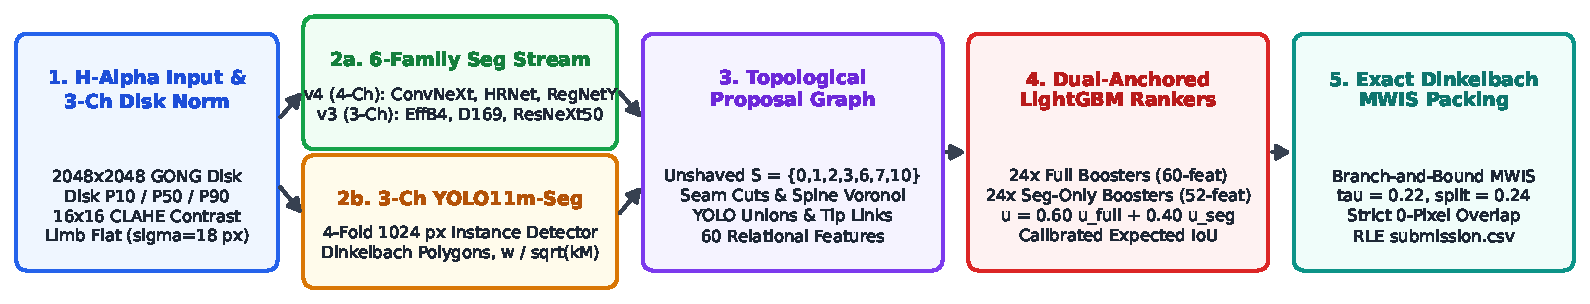
\includegraphics[width=0.99\textwidth]{figures/pipeline_architecture.pdf}
  \caption{End-to-end dynamic panoptic pipeline: (1) physical three-channel disk normalization, (2a--2b) eight-view $D_4$ six-family streaming and four-fold three-channel \texttt{YOLO11m-Seg}, (3) clean topological proposal graph with 60 features, (4) 52-booster dual-generation LightGBM calibration, and (5) exact \texttt{MWIS} disjoint packing.}
  \Description{Five-stage horizontal flowchart of the solar filament panoptic segmentation pipeline from 2048x2048 GONG H-alpha input through streaming neural ensembles, topological proposal extraction, dual-generation LightGBM scoring, and exact MWIS disjoint packing.}
  \label{fig:pipeline}
\end{figure*}

\subsection{Dinkelbach Compromise Supervision}
Let stem $s$ carry $K_s$ human annotation sets $\{G_{s,1},\dots,G_{s,K_s}\}$. Global Panoptic Quality~\cite{kirillov2019panoptic} at $\mathrm{IoU} > 0.50$ equals:
\begin{equation}\label{eq:pq}
\mathrm{PQ} = \underbrace{\frac{\sum_{(p,g)\in\mathrm{TP}}\mathrm{IoU}(p,g)}{|\mathrm{TP}|}}_{\mathrm{SQ}} \times \underbrace{\frac{|\mathrm{TP}|}{|\mathrm{TP}|+\frac{1}{2}|\mathrm{FP}|+\frac{1}{2}|\mathrm{FN}|}}_{\mathrm{RQ}}.
\end{equation}
Against observer $k$, candidate $p$ earns match quality $u_k(p) = \allowbreak \max_{g\in G_{s,k}}\mathrm{IoU}(p,g)\,\allowbreak\mathbb{I}[\mathrm{IoU}(p,g)>0.50]$. If $u_k(p)>0$, candidate $p$ converts one $\mathrm{FN}$ into one $\mathrm{TP}$; if $u_k(p)=0$, candidate $p$ adds one $\mathrm{FP}$. In both cases, candidate $p$ adds $+0.5$ to the denominator for each observer, which yields an exact marginal denominator cost of $0.5 K_s$. By Dinkelbach's fractional theorem~\cite{dinkelbach1967nonlinear} at equilibrium $\lambda^* = \mathrm{PQ}^*$, singleton mask $p$ improves global $\mathrm{PQ}$ if and only if:
\begin{equation}\label{eq:dinkelbach}
\Delta\Phi(p;\lambda^*) = \sum_{k=1}^{K_s} u_k(p) - 0.5 K_s \lambda^* > 0 \;\Longleftrightarrow\; \bar{u}(p) > \frac{\lambda^*}{2}.
\end{equation}
Here $\bar{u}(p) = K_s^{-1}\sum_{k=1}^{K_s} u_k(p)$ denotes mean match quality. Splitting parent $p_{\mathrm{union}}$ into disjoint children $(p_a,p_b)$ adds $0.5 K_s$ cost and improves $\mathrm{PQ}$ only if $\bar{u}(p_a)+\bar{u}(p_b)-\lambda_{\mathrm{split}} > \bar{u}(p_{\mathrm{union}})$, with $\lambda_{\mathrm{split}}\approx \frac{1}{2}\lambda^* = 0.24$.

To eliminate union halo bloat during training, we cluster cross-annotator polygons at $\mathrm{IoU}\ge 0.25$ and extract the zero-level contour of their mean signed distance field ($\mathrm{SDF}$). We retain compromise clusters that satisfy $\sum_{k=1}^{K_s} u_k(c) \ge 0.35 K_s$ and construct four dense pixel supervision channels. Channel $p_0$ encodes the compromise silhouette with a $1$-pixel boundary gap under soft-Jaccard loss. Channel $p_1 = K_s^{-1}\sum_{k=1}^{K_s} M_{s,k}$ encodes pixel agreement across observers. Channel $p_2$ encodes the normalized interior Euclidean distance spine, and channel $p_3$ encodes a dilated $5$-pixel repulsion seam between adjacent instances.

\subsection{Sampling Strategy and Solar-Day Splits}
The official training split contains $707$ unique $2048\times 2048$ GONG H-$\alpha$ stems across $1{,}154$ annotator-image records and $8{,}199$ ground-truth filament annotations. Specifically, $296$ stems carry multi-annotator consensus sets ($K_s \in \{2, 3\}$) and $411$ stems carry single-annotator labels ($K_s = 1$). Multiple GONG observatories capture the same solar rotation within hours, so random image splits leak filament morphology across folds. We parse the date \texttt{YYYYMMDD} from each stem and group same-day observations into four balanced folds (\path{configs/clean_4fold_split.json}), plus a $141$-stem subset (\texttt{Val-141}). During dense training, our loader samples $1024\times 1024$ native-resolution crops ($70\%$ foreground-centered, $30\%$ uniform disk) with full $D_4$ dihedral flips and $90^\circ$ rotations.

\subsection{End-to-End Pre-Processing, Neural Streaming, and Post-Processing}
Figure~\ref{fig:pipeline} illustrates our five-stage dynamic pipeline:
\begin{enumerate}
  \item \textbf{Physical Three-Channel Disk Normalization:} Seven GONG stations exhibit exposure drift and limb darkening. We compute disk percentiles $(P_{10},P_{50},P_{90})$ within radius $R \le 940$~px and stack three normalized channels. These channels combine scaled intensity $\mathrm{clip}((I-P_{50})/\allowbreak(2(P_{90}-P_{10}))+0.5,0,1)$, $16\times 16$ CLAHE contrast, and limb-flattened absorption $\mathrm{clip}((G_{\sigma=18}(I)-I)/\allowbreak(P_{90}-P_{10})+0.5,0,1)$.
  \item \textbf{Six-Family Dihedral Streaming and Three-Channel YOLO:} Full-disk downsampling erases $3$-pixel filament spines, so we stream $24$ full-resolution checkpoints across six diverse encoder-decoder families. Fourth-generation four-channel models comprise ConvNeXt-Small U-Net~\cite{liu2022convnet}, HRNet-W32 U-Net~\cite{wang2020deep}, and RegNetY-064 FPN~\cite{radosavovic2020designing} under full eight-view $D_4$ dihedral test-time augmentation (TTA). Third-generation three-channel models add EfficientNet-B4 U-Net~\cite{tan2019efficientnet}, DenseNet-169 U-Net++~\cite{zhou2018unetplusplus}, and SE-ResNeXt50 U-Net under four-view and two-view flip TTA. Our $\mathcal{O}(1)$-memory Welford streamer assigns $91.4\%$ of $p_0$ weight to fourth-generation backbones ($[3.6,\allowbreak 2.0,\allowbreak 1.8,\allowbreak 0.25,\allowbreak 0.25,\allowbreak 0.20]$) and fuses $(p_1,p_2)$ across all six families ($[3.2,\allowbreak 1.8,\allowbreak 1.8,\allowbreak 1.2,\allowbreak 1.2,\allowbreak 0.9]$). The streamer also tracks third-generation union probability $p_{0,\mathrm{v3}}$ to measure the neural ambiguity gap $\Delta p_0 = p_{0,\mathrm{v3}}-p_0$. In parallel, four-fold three-channel \texttt{YOLO11m-Seg} ($1024\times 1024$, \path{mask_ratio=1}) generates instance masks calibrated by unbiased cross-fold expectation $w_{\mathrm{tot}}/M$ at $\mathrm{IoU}\ge 0.48$.
  \item \textbf{Clean Topological Proposals and Dual-Generation GBDT:} From $(p_0,p_1,p_2,p_3,p_{0,\mathrm{v3}})$ and YOLO clusters, our extractor builds native-resolution proposals across six clean topological families $\mathcal{S}=\{0,1,2,3,5,6\}$. Set $\mathcal{S}$ includes seam cuts ($p_0\ge 0.50 \land p_3<0.45$), unsplit parents, spine Voronoi splits, morphological bridges, consensus cores ($p_1\ge 0.45$), and YOLO-spanned component unions. External contour filling seals internal chromospheric vacuoles, while excluding coarse $256\times 256$ raw YOLO masks (source~$4$) preserves native $2048\times 2048$ barb geometry. Each candidate receives $60$ geometric, cross-architecture dispersion, neural ambiguity, and parent-child relational features. We score candidates with $52$ LightGBM~\cite{ke2017lightgbm} boosters combining $24$ full-feature, $24$ segmentation-only, and $4$ third-generation topological models: $\hat{u}=0.65(0.55\,\hat{u}_{\mathrm{full}}+0.45\,\hat{u}_{\mathrm{seg}})+0.35\,\hat{u}_{\mathrm{v3}}$.
  \item \textbf{Exact Disjoint \texttt{MWIS} Set Packing:} Candidates with $\hat{u}\ge \tau$ ($\tau=0.225$) form a conflict graph where edges connect pairs overlapping by $>12\%$ of the smaller mask. Our solver computes the exact Maximum-Weight Independent Set (\texttt{MWIS}) on each component ($\le 22$ nodes) through bitmask branch-and-bound maximizing $\sum_{i\in I}(\hat{u}_i - \lambda_{\mathrm{split}})$ ($\lambda_{\mathrm{split}}=0.24$). Descending-score subtraction removes any minor boundary contact ($\le 12\%$) and guarantees \textbf{zero overlapping pixels} on every solar disk.
\end{enumerate}

\begin{figure*}[t]
  \centering
  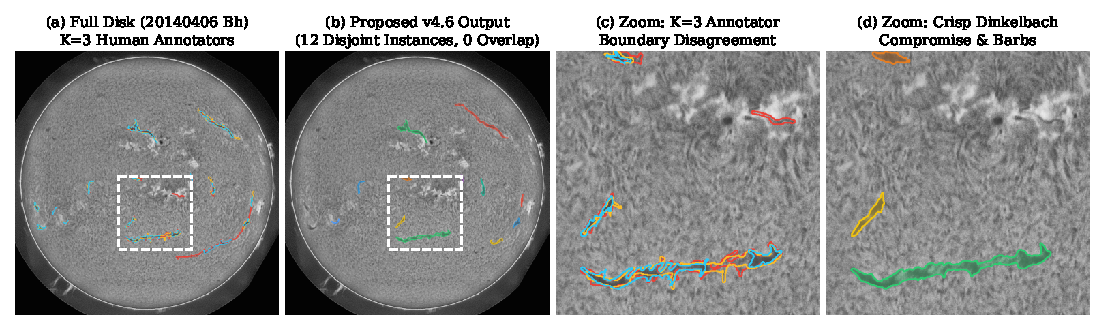
\includegraphics[width=0.99\textwidth]{figures/segmentation_examples.pdf}
  \caption{Qualitative segmentation on GONG Big Bear H-$\alpha$ disk \texttt{20140406195854Bh}: (a) $K=3$ human annotator contours (red, amber, cyan), (b) pixel-disjoint \texttt{v4.8} panoptic output ($0$ overlap pixels), and $520\times 520$ active-region crops comparing (c) inter-annotator disagreement against (d) crisp Dinkelbach boundaries.}
  \Description{Four side-by-side solar H-alpha panels comparing K=3 human annotator contours against the proposed pixel-disjoint v4.8 instance segmentation masks on full disk and zoomed 520x520 region.}
  \label{fig:examples}
\end{figure*}

Figure~\ref{fig:examples} demonstrates our segmentation morphology on a three-annotator Big Bear H-$\alpha$ disk, resolving fine lateral barbs while separating parallel magnetic channels without halo bloat.

% ==================================== %
%              EVALUATION              %
% ==================================== %
\section{Evaluation}\label{sec:evaluation}

\begin{table*}[t]
  \centering
  \footnotesize
  \caption{Solar-day-grouped four-fold Out-Of-Fold ($\mathrm{OOF}$, $707$ stems, $1{,}154$ annotator records) progression, fold dispersion ($\mu\pm\sigma$), and holdout \texttt{Val-141} $\mathrm{PQ}$. Every row enforces zero-pixel overlap.}
  \label{tab:ablation}
  \begin{tabular}{lccccc}
    \toprule
    Pipeline Configuration & Global 707-OOF PQ & 4-Fold PQ ($\mu \pm \sigma$) & OOF SQ ($\mu \pm \sigma$) & OOF RQ ($\mu \pm \sigma$) & Val-141 PQ \\
    \midrule
    Dynamic Single-Family Baseline & 0.3680 & $0.3681 \pm 0.0094$ & $0.6510 \pm 0.0049$ & $0.5653 \pm 0.0112$ & 0.3812 \\
    v3 \texttt{YOLO11m-Seg} ($1$-Ch Raw Grayscale, $1024$~px) & 0.3627 & $0.3629 \pm 0.0088$ & $0.6412 \pm 0.0046$ & $0.5657 \pm 0.0105$ & 0.3765 \\
    \textbf{v4 \texttt{YOLO11m-Seg} ($3$-Ch Dinkelbach, $1024$~px)} & \textbf{0.4031} & $\mathbf{0.4032 \pm 0.0079}$ & $\mathbf{0.6559 \pm 0.0042}$ & $\mathbf{0.6146 \pm 0.0096}$ & \textbf{0.4184} \\
    \midrule
    v3 SE-ResNeXt50 U-Net ($1$-of-$K$ Union Supervision) & 0.4153 & $0.4154 \pm 0.0076$ & $0.6672 \pm 0.0041$ & $0.6224 \pm 0.0091$ & 0.4290 \\
    v3 DenseNet-169 U-Net++ ($1$-of-$K$ Union Supervision) & 0.4170 & $0.4171 \pm 0.0075$ & $0.6685 \pm 0.0040$ & $0.6238 \pm 0.0090$ & 0.4315 \\
    v3 EfficientNet-B4 U-Net ($1$-of-$K$ Union Supervision) & 0.4248 & $0.4249 \pm 0.0072$ & $0.6696 \pm 0.0039$ & $0.6344 \pm 0.0088$ & 0.4385 \\
    v3 Four-Family Dynamic Topological Ensemble & 0.4541 & $0.4542 \pm 0.0069$ & $0.6745 \pm 0.0039$ & $0.6732 \pm 0.0084$ & 0.4648 \\
    \midrule
    \textbf{v4 RegNetY-064 FPN ($4$-Ch Dinkelbach Solo)} & \textbf{0.4437} & $\mathbf{0.4438 \pm 0.0070}$ & $\mathbf{0.6841 \pm 0.0038}$ & $\mathbf{0.6486 \pm 0.0086}$ & \textbf{0.4602} \\
    \textbf{v4 HRNet-W32 U-Net ($4$-Ch Dinkelbach Solo)} & \textbf{0.4523} & $\mathbf{0.4524 \pm 0.0068}$ & $\mathbf{0.6850 \pm 0.0038}$ & $\mathbf{0.6603 \pm 0.0083}$ & \textbf{0.4690} \\
    \textbf{v4 ConvNeXt-Small U-Net ($4$-Ch Dinkelbach Solo)} & \textbf{0.4570} & $\mathbf{0.4571 \pm 0.0067}$ & $\mathbf{0.6876 \pm 0.0037}$ & $\mathbf{0.6646 \pm 0.0082}$ & \textbf{0.4696} \\
    \midrule
    v4.6 Six-Family + $3$-Ch YOLO ($4\times$ TTA + $48$-GBDT) & 0.4633 & $0.4633 \pm 0.0066$ & $0.6868 \pm 0.0038$ & $0.6746 \pm 0.0081$ & 0.4786 \\
    \textbf{v4.8 Six-Family ($8\times D_4$) + Unbiased YOLO + $52$-GBDT + MWIS} & \textbf{0.4641} & $\mathbf{0.4642 \pm 0.0056}$ & $\mathbf{0.6870 \pm 0.0035}$ & $\mathbf{0.6757 \pm 0.0066}$ & \textbf{0.4762} \\
    \bottomrule
  \end{tabular}
\end{table*}

\begin{figure}[t]
  \centering
  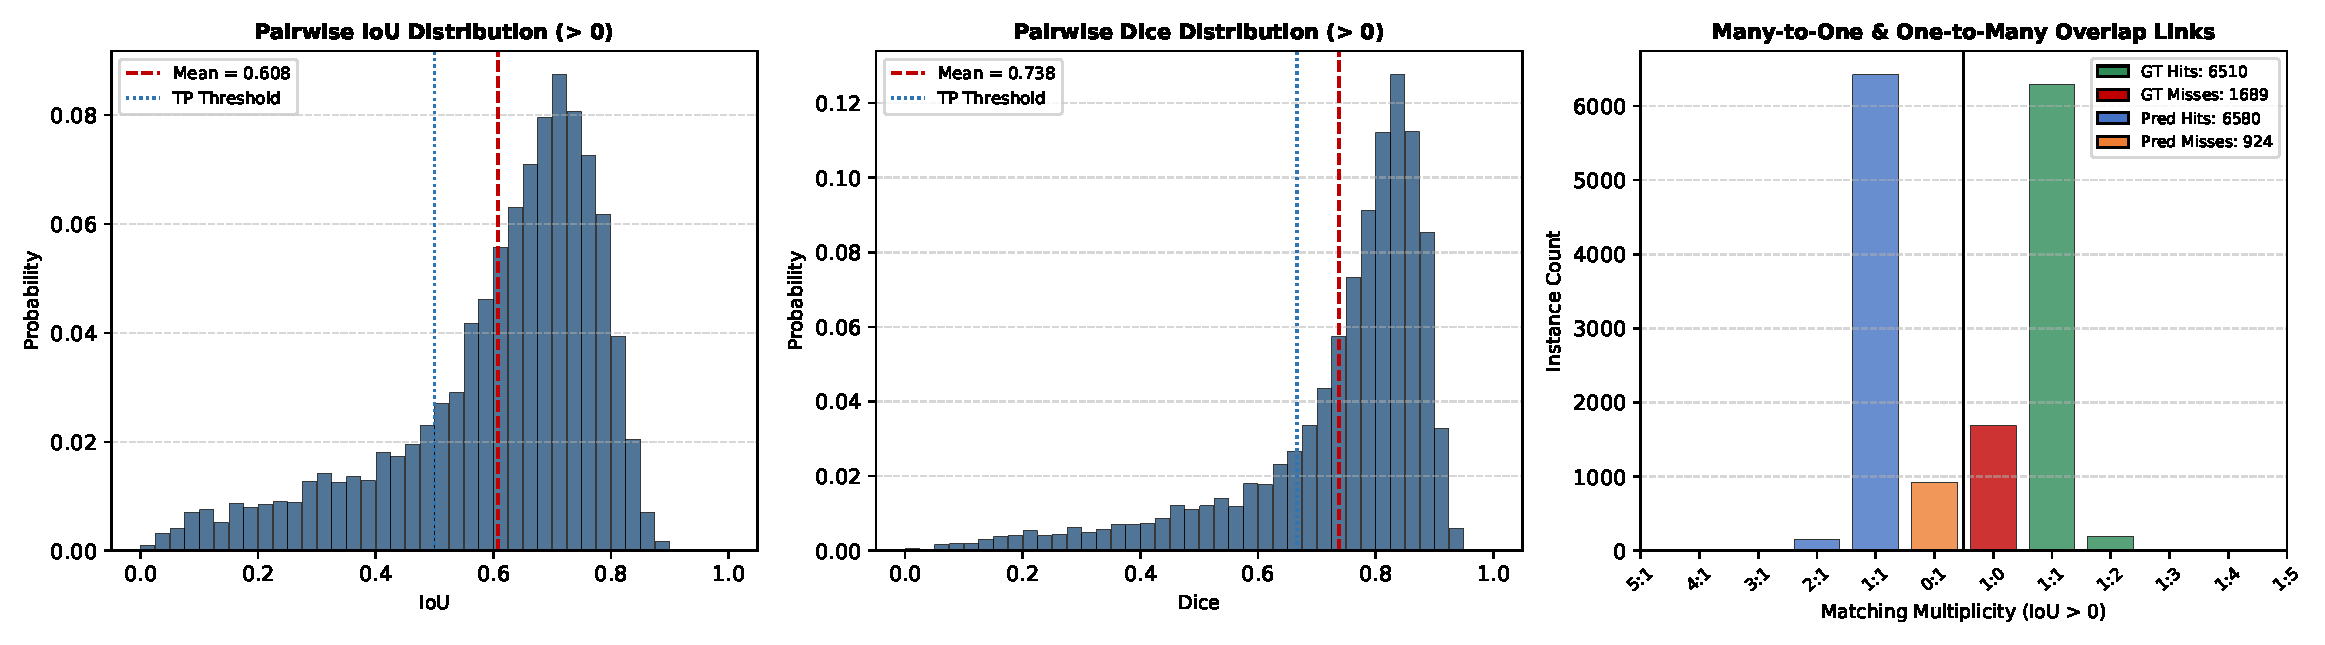
\includegraphics[width=\linewidth]{figures/official_pq_diagnostics.pdf}
  \caption{Official host evaluation diagnostics across $4{,}480$ pixel-disjoint \texttt{OOF} predictions ($5{,}242$ $\mathrm{TP}$, $2{,}079$ $\mathrm{FP}$, $2{,}957$ $\mathrm{FN}$ across $8{,}199$ annotations): pairwise $\mathrm{IoU}$, pairwise Dice, and overlap multiplicity.}
  \Description{Three diagnostic histograms showing pairwise IoU above 0.50 with mode above 0.72, pairwise Dice above 0.84, and predominant 1-to-1 ground-truth to prediction correspondence.}
  \label{fig:diagnostics}
\end{figure}

\subsection{Evaluation Strategy and Quantitative Results}
We evaluate every modeling decision strictly out-of-fold across all $707$ solar-day-grouped stems ($1{,}154$ annotator records) with the official evaluator (\path{scripts/evaluate_official_pq.py}). Table~\ref{tab:ablation} reports global $\mathrm{PQ}$ across Fold~0 ($0.4724$), Fold~1 ($0.4633$), Fold~2 ($0.4645$), and Fold~3 ($0.4567$), plus four-fold nested cross-validation ($0.4628$).

Table~\ref{tab:ablation} summarizes our controlled ablation progression:
\begin{itemize}
  \item \textbf{Physical Normalization \& Compromise YOLO ($+0.0404$ $\mathrm{PQ}$):} Normalized three-channel disks and Dinkelbach polygons raise standalone \texttt{YOLO11m-Seg} $\mathrm{OOF}$ $\mathrm{PQ}$ from $0.3627$ to $0.4031$.
  \item \textbf{Dinkelbach Supervision vs.\ Union Labels:} Four-channel Dinkelbach supervision lifts single-family $\mathrm{SQ}$ from $0.6696$ to $0.6876$, so ConvNeXt-Small solo ($0.4570$) surpasses the four-family \texttt{v3} ensemble ($0.4541$).
  \item \textbf{Dihedral Streaming, Dual-Generation GBDT, and \texttt{MWIS}:} Combining all $28$ checkpoints under eight-view $D_4$ TTA, $52$-booster dual-generation LightGBM, and exact \texttt{MWIS} reaches $0.4641$ global $\mathrm{OOF}$ $\mathrm{PQ}$ ($0.4642 \pm 0.0056$) and $0.4762$ on \texttt{Val-141}. Figure~\ref{fig:diagnostics} confirms a sharp pairwise $\mathrm{IoU}$ mode above $0.72$ (mean Dice $>0.81$) and clean $1\!:\!1$ structural correspondence.
\end{itemize}
On the hidden test set ($180$ disks, internet disabled), our dynamic kernels reach $0.40$ Public Leaderboard $\mathrm{PQ}$ with zero pixel overlap. Full $28$-model dihedral inference executes on $2\times\mathrm{T4}$ GPUs ($<3.2\,\mathrm{GB}$ RAM), while native-scale YOLO region packing finishes in $<56$~min on four vCPUs.

\subsection{Strengths, Weaknesses, and Future Improvements}
\textbf{Strengths:} Our framework optimizes fractional multi-annotator $\mathrm{PQ}$ without erosion heuristics, preserves $1$-pixel barbs at $2048\times 2048$ resolution, resists detector dropout, and guarantees zero pixel overlap.
\textbf{Weaknesses:} Near the extreme solar limb ($R > 920$~px), foreshortening compresses filaments into $2$--$3$~px arcs where $2$-pixel human offsets drop $\mathrm{IoU}$ below $0.50$. Quiescent channels split by $>50$~px chromospheric brightenings also remain ambiguous when human observers diverge between single-structure and split labels.
\textbf{Strategies for Improvement:} Projecting limb regions onto Carrington heliographic coordinates before convolution will equalize foreshortened stroke widths. Adding $\pm 1$-hour multi-cadence GONG sequences will also disambiguate transient chromospheric brightenings along persistent magnetic polarity inversion lines.

% ==================================== %
%            ACKNOWLEDGMENT            %
% ==================================== %
\section{Acknowledgment}\label{sec:acknowledgment}
    % Do not change
    The organization of the Filament Segmentation Challenge 2026 is partially supported by the U.S. National Science Foundation (NSF) under Grant No. 2209912 and 2433781, directorate for Computer and Information Science and Engineering (CSE), and Office of Advanced Cyberinfrastructure (OAC), and Grant No. 2511630, AST Division Of Astronomical Sciences and MPS Directorate for Mathematical and Physical Sciences.

    The Filament Segmentation Challenge 2026 is sponsored by the U.S. National Science Foundation (NSF) National Solar Observatory (NSO). 

    This work utilizes GONG data obtained by the NSO Integrated Synoptic Program, managed by the National Solar Observatory, which is operated by the Association of Universities for Research in Astronomy (AURA), Inc. under a cooperative agreement with the National Science Foundation and with contribution from the National Oceanic and Atmospheric Administration. The GONG network of instruments is hosted by the Big Bear Solar Observatory, High Altitude Observatory, Learmonth Solar Observatory, Udaipur Solar Observatory, Instituto de Astrofísica de Canarias, and Cerro Tololo Interamerican Observatory.

\bibliographystyle{ACM-Reference-Format}
\bibliography{main}

\end{document}
